\documentclass[a4paper, 12pt]{article}
\usepackage[utf8]{inputenc}
\usepackage[english,russian]{babel}
\usepackage[warn]{mathtext}
\usepackage{graphicx}
\usepackage{float}
\usepackage{multirow}
\restylefloat{table}
\usepackage{amsmath}
\usepackage{floatflt}
\usepackage[T2A]{fontenc}
\usepackage[left=20mm, top=20mm, right=20mm, bottom=20mm, footskip=10mm]{geometry}

\tolerance 1414
\hbadness 1414
\emergencystretch 1.5em
\hfuzz 0.3pt        % размер максимального переполнения без warning'a
\widowpenalty=10000 % запрещает одиночную строку абзаца в начале страницы
\vfuzz \hfuzz
\raggedbottom       % если на странице мало содержимого, добавить пустое место в конце, а не в середине страницы



\begin{document}

\begin{titlepage}
	\centering
	\vspace{5cm}
	{\scshape\LARGE московский физико-технический институт (национальный исследовательский университет) \par}
	\vspace{6cm}
	{\scshape\Large Лабораторная работа 4.1.1 \par}
	{\huge\bfseries Оптические системы \par}
	\vspace{1cm}
	\vfill
\begin{flushright}
	{\large Б03-102}\par
	\vspace{0.3cm}
	{\LARGE Куланов Александр}
\end{flushright}
	

	\vfill


	Долгопрудный, 2023 г.
\end{titlepage}

\begin{itemize}
	\item \textbf{Цель работы:} Изучение различных оптических систем
    \item \textbf{В работе используются:} оптическая скамья с набором рейтеров, положительные и отрицательные линзы,  экран, осветитель, зрительная труба, светофильтры, кольцевые диафрагмы.
\end{itemize}

\section{Теоретические сведения}
\subsection{Определения фокусных расстояний по формуле тонкой линзы}

В настоящей работе пользуемся приближением, что линзы тонкие (что в общем-то не так). Для тонкой линзы справедливо:

\begin{equation}
	\frac{1}{f}	= \frac{1}{a} + \frac{1}{b},
\end{equation}
где $a$ - расстояние до предмета, $b$ - расстояние до изображения, $f$ - фокусное расстояние линзы. 

\subsection{Определения фокусных расстояний с помощью зрительной трубы}

Настроим зрительную трубу на бесконечность. Тогда при помещении линзы на расстоянии от источника, равном фокусному, в зрительной трубе можно видеть четкое изображение. Такой метод годится
только для положительной линзы. Чтобы найти фокус отрицательной линзы, нужно чтобы расстояние $a$ совпадло с модулем фокусного расстояния этой отрицательной линзы (рис. \ref{fig:ris1})

\begin{figure}[H]
    \centering
    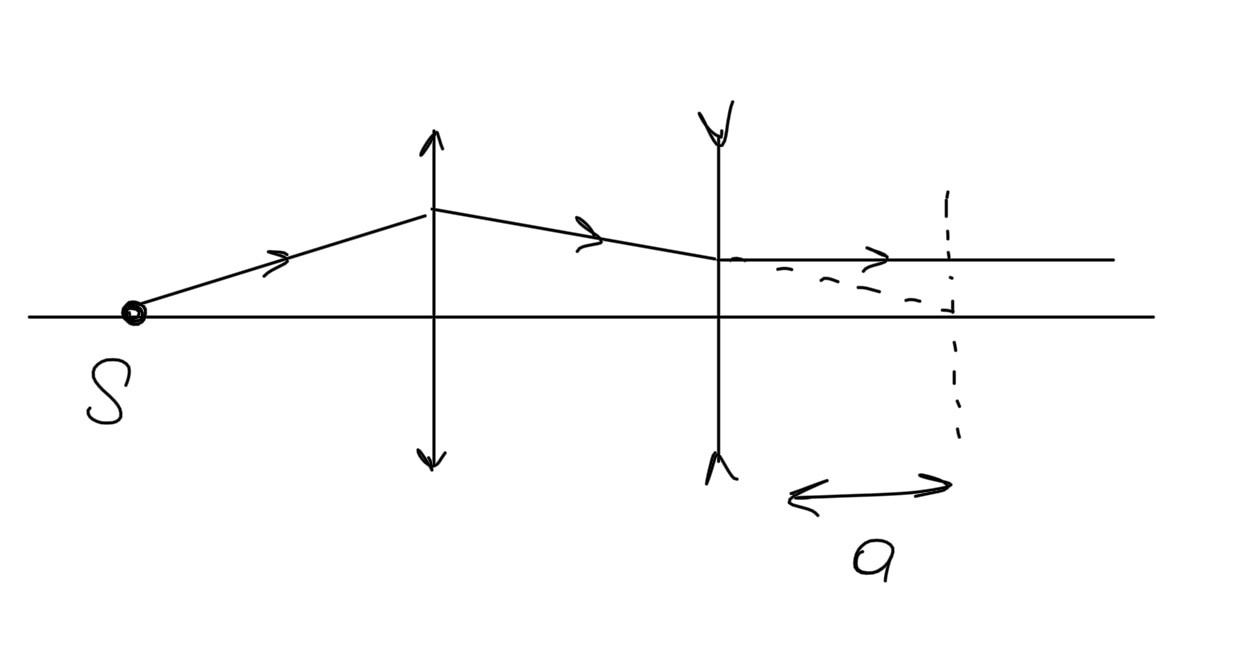
\includegraphics[width=1\textwidth]{ris1}
    \caption{Ход лучей в системе с отрицательной линзой}
    \label{fig:ris1}
\end{figure}

\subsection{Определения фокусных расстояний с помощью метода Бесселя}

\begin{figure}[H]
    \centering
    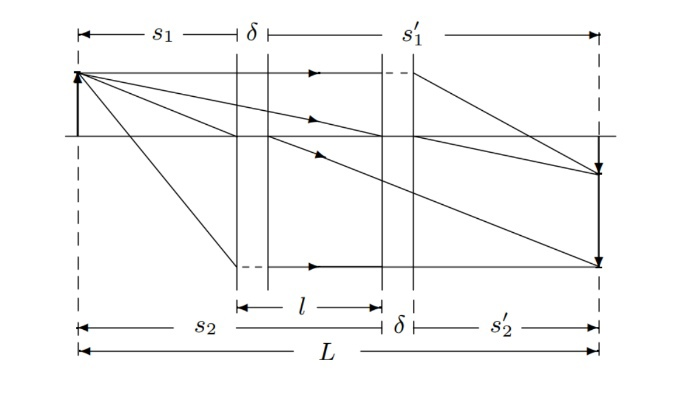
\includegraphics[width=1\textwidth]{bessel.jpg}
    \caption{Схема Бесселя}
    \label{fig:ris3}
\end{figure}

Для метода Бесселя имеем уравнение:
\begin{equation}
	-\frac{1}{s} + \frac{1}{L - \delta + s} = \frac{1}{f}
\end{equation}
При $L > 4f + \delta $ решения этого уравнения $s_1$, $s_2$ показаны на рис. {\ref{fig:ris3}}. С учетом симметрии $L - \delta = s^{'}_1 - s_1, l = -s_2 + s_1 = s_1 + s^{'}_1$. Откуда

\begin{equation}
	f = \frac{(L - \delta)^2 - l^2}{4(L - \delta)}
\end{equation}

\subsection{Моделирование телескопа}

Соберём телескоп из двух собирающих линз. Третью линзу поставим перед телескопом, чтобы получить параллельный пучёк света. 

\begin{figure}[H]
    \centering
    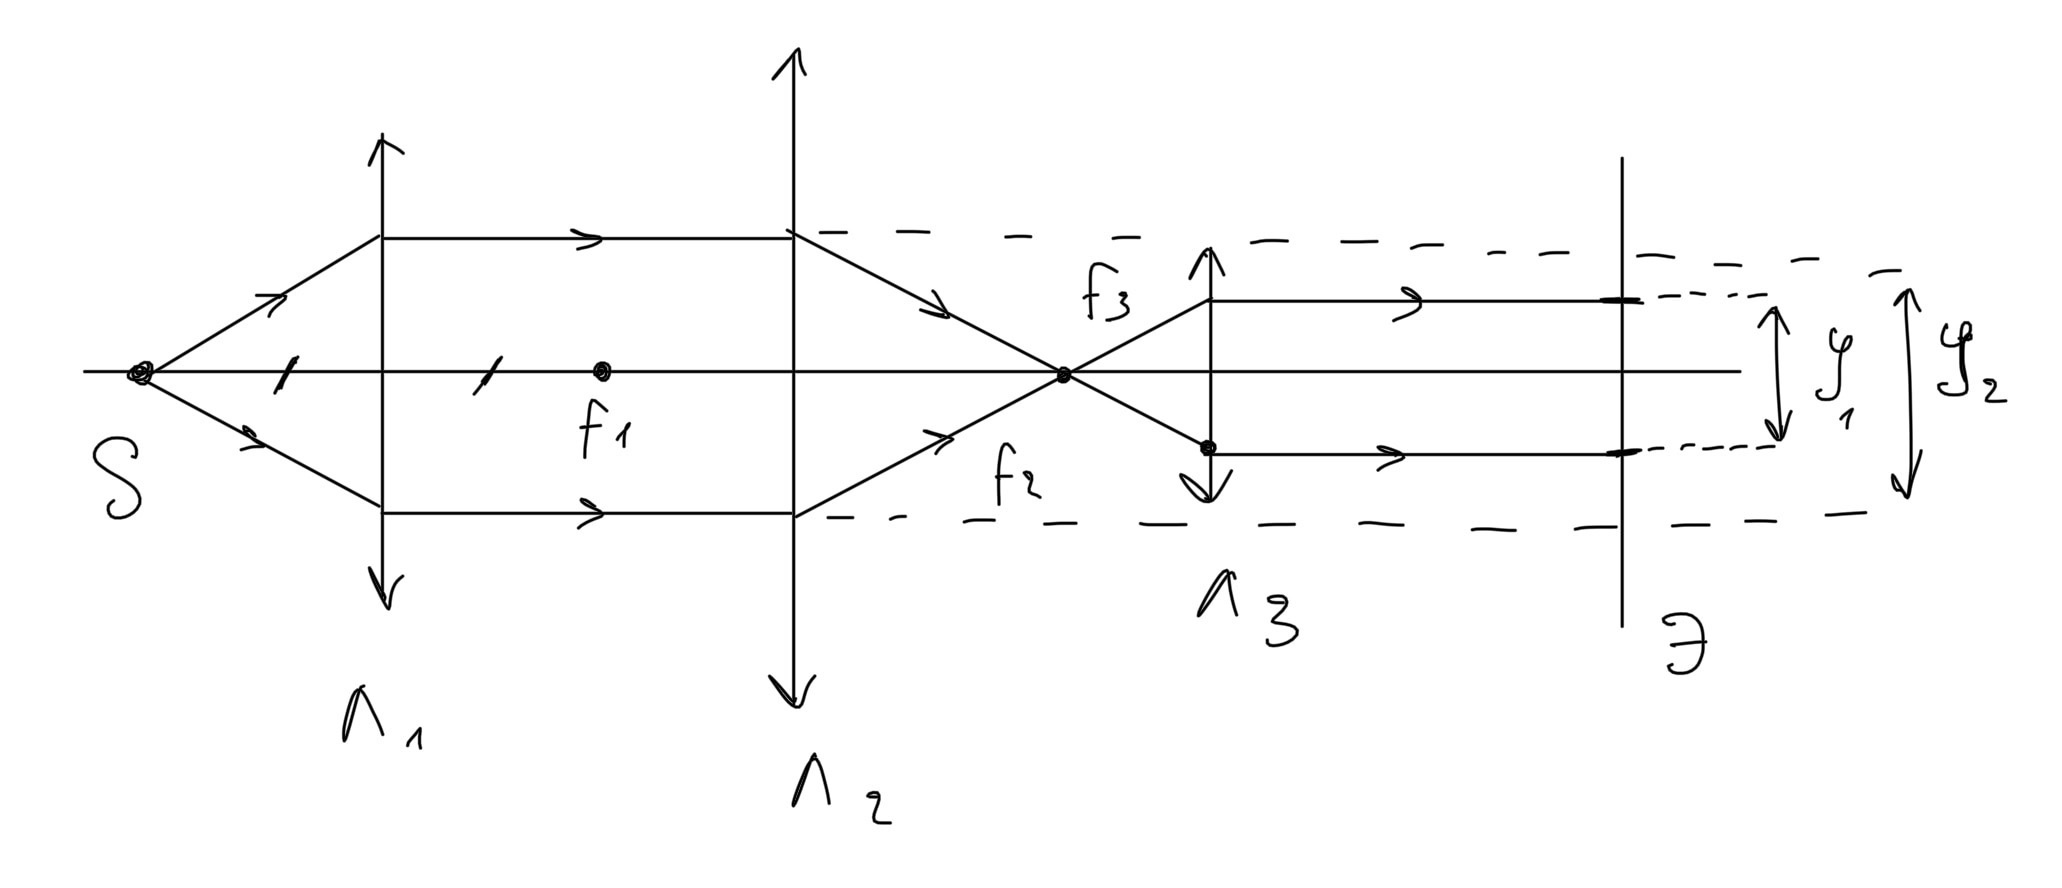
\includegraphics[width=1\textwidth]{telescope.jpg}
    \caption{Схема телескопа}
    \label{fig:ris2}
\end{figure}

В работе интересно проверить соотношение:

\begin{equation}
	\frac{y_2}{y_1} = \frac{f_2}{f_3}
\end{equation}

\section{Обработка результатов}

\subsection{Определения фокусных расстояний по формуле тонкой линзы}
Для двух собирающих линз роведем серию экспериментов, меняя каждый раз $a$ и $b$. Построим графики зависимости $1/a$ от $1/b$. Тогда обратная величина коэффициента наклона будет фокусным расстоянием.

\begin{figure}[H]
    \centering
    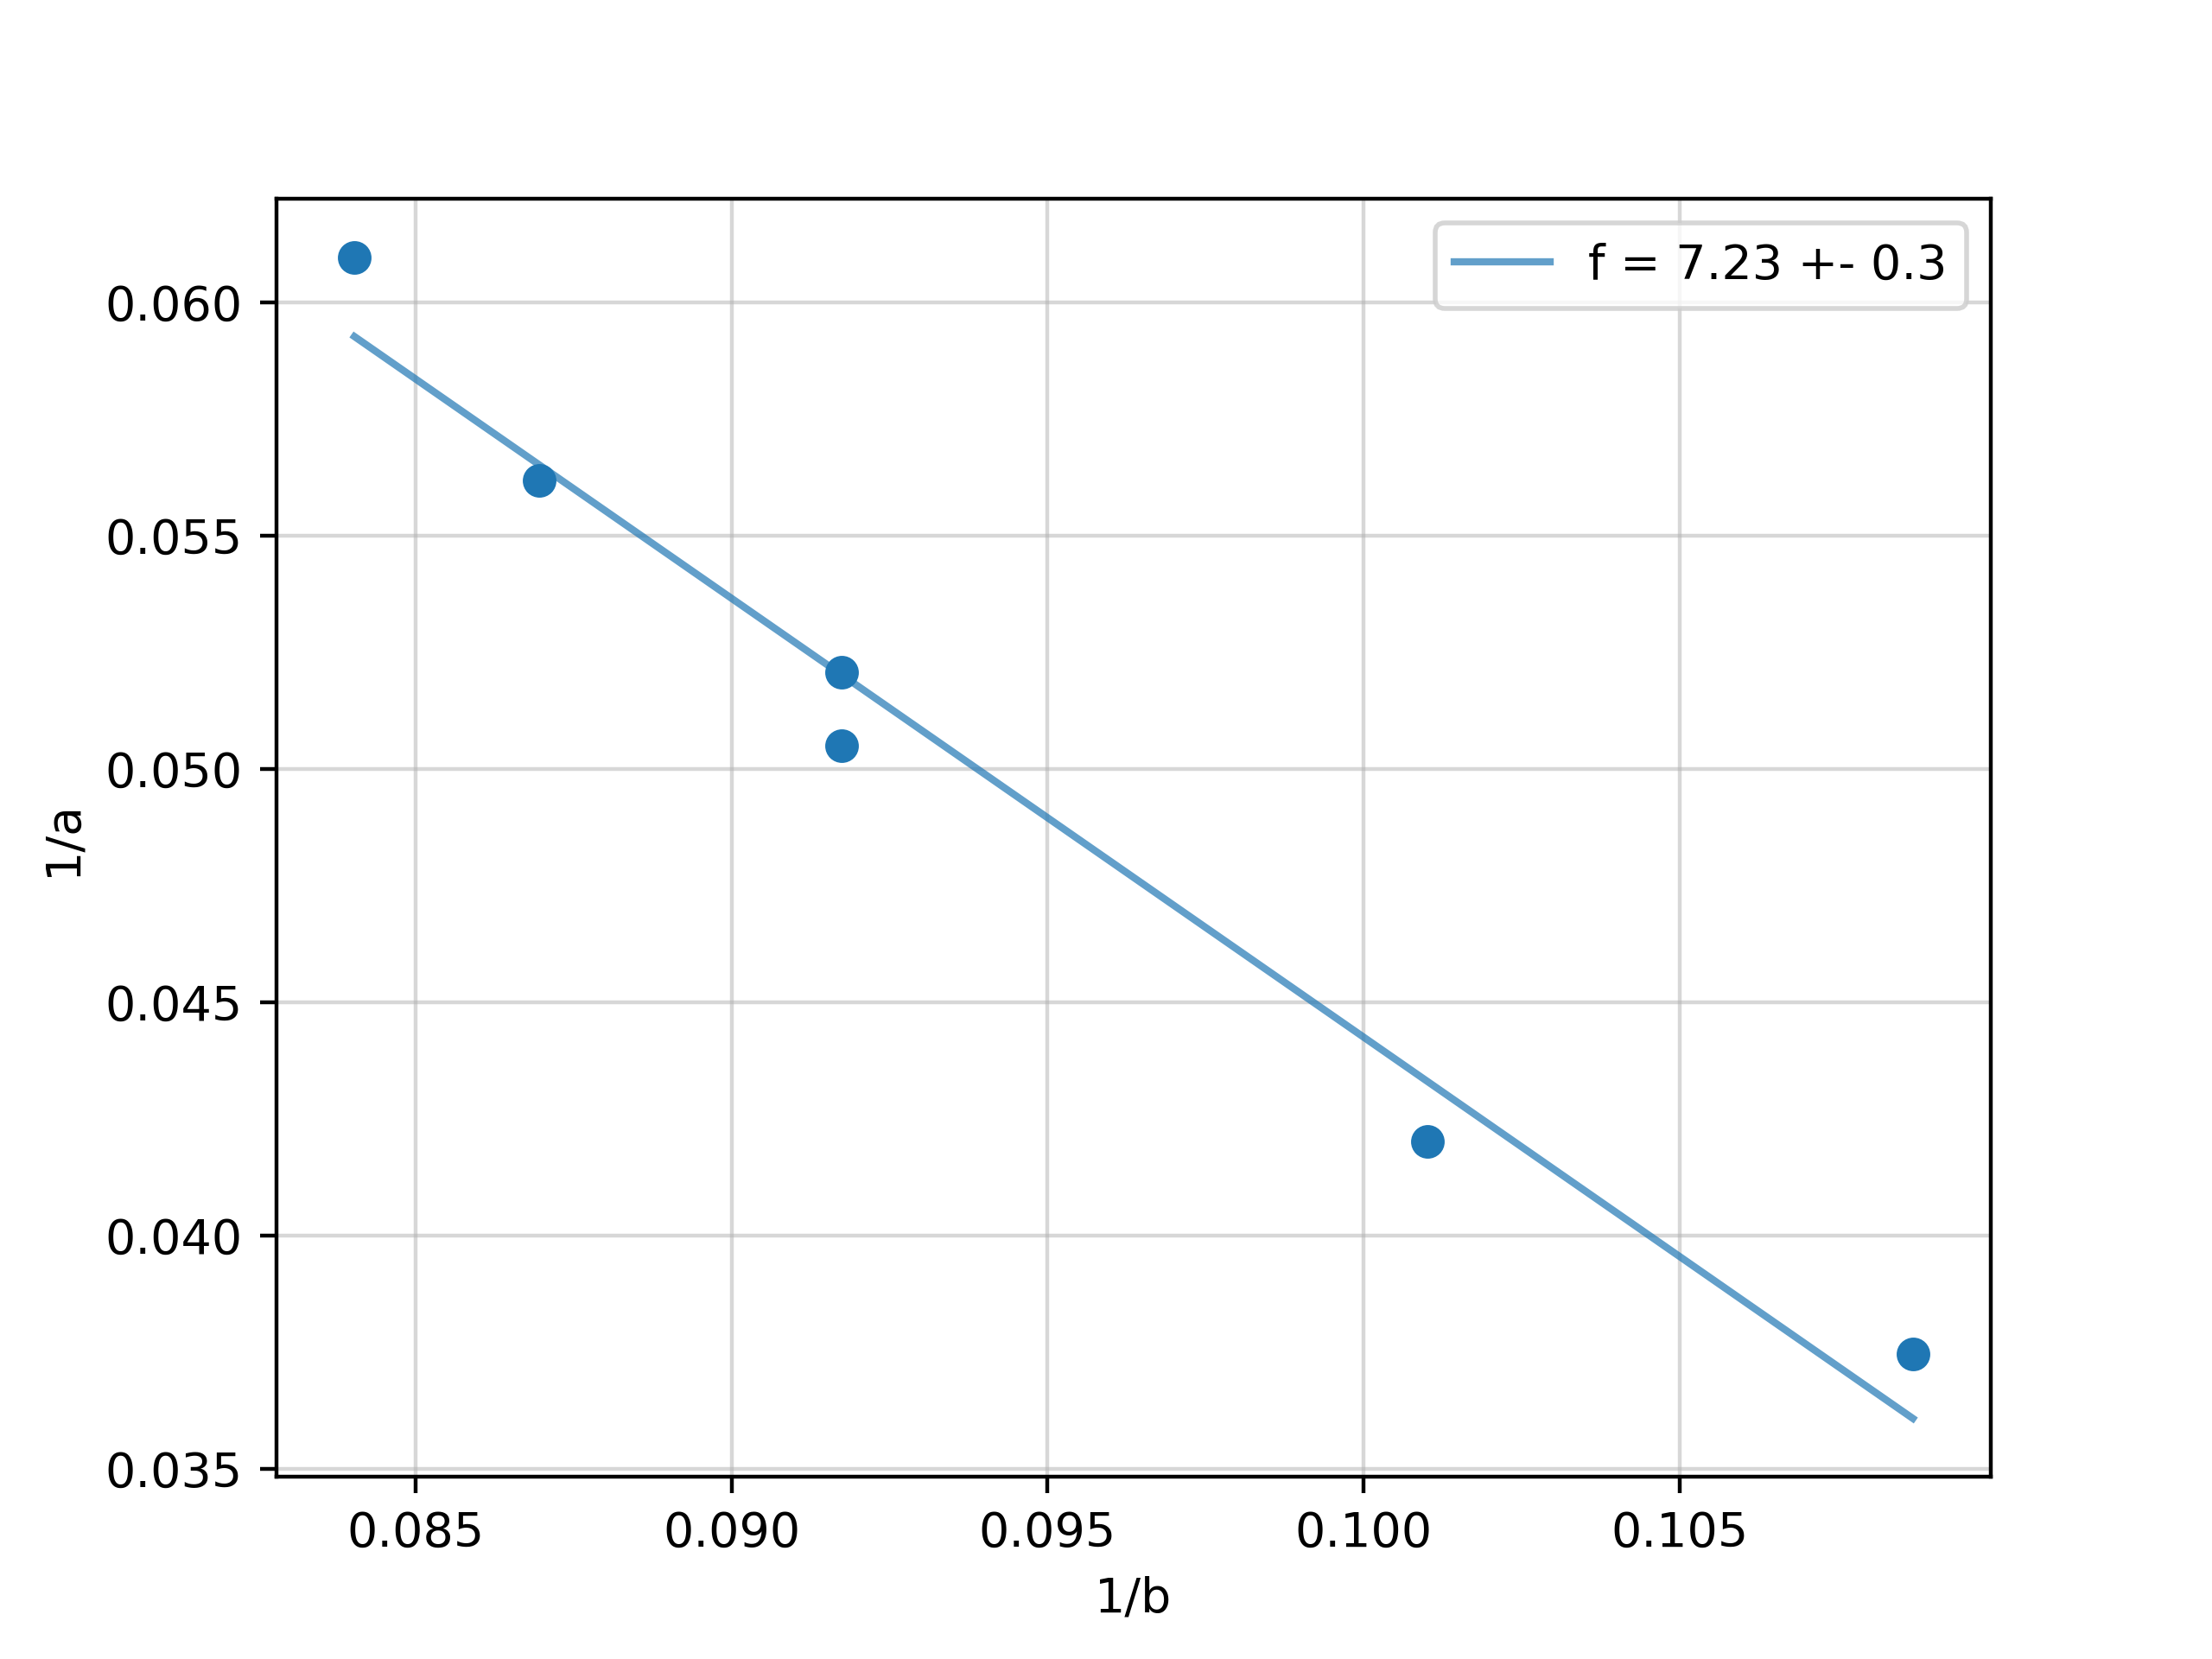
\includegraphics[width=1\textwidth]{plot1.png}
    \caption{$f(1/a)$}
    \label{fig:plot1}
\end{figure}

\begin{figure}[H]
    \centering
    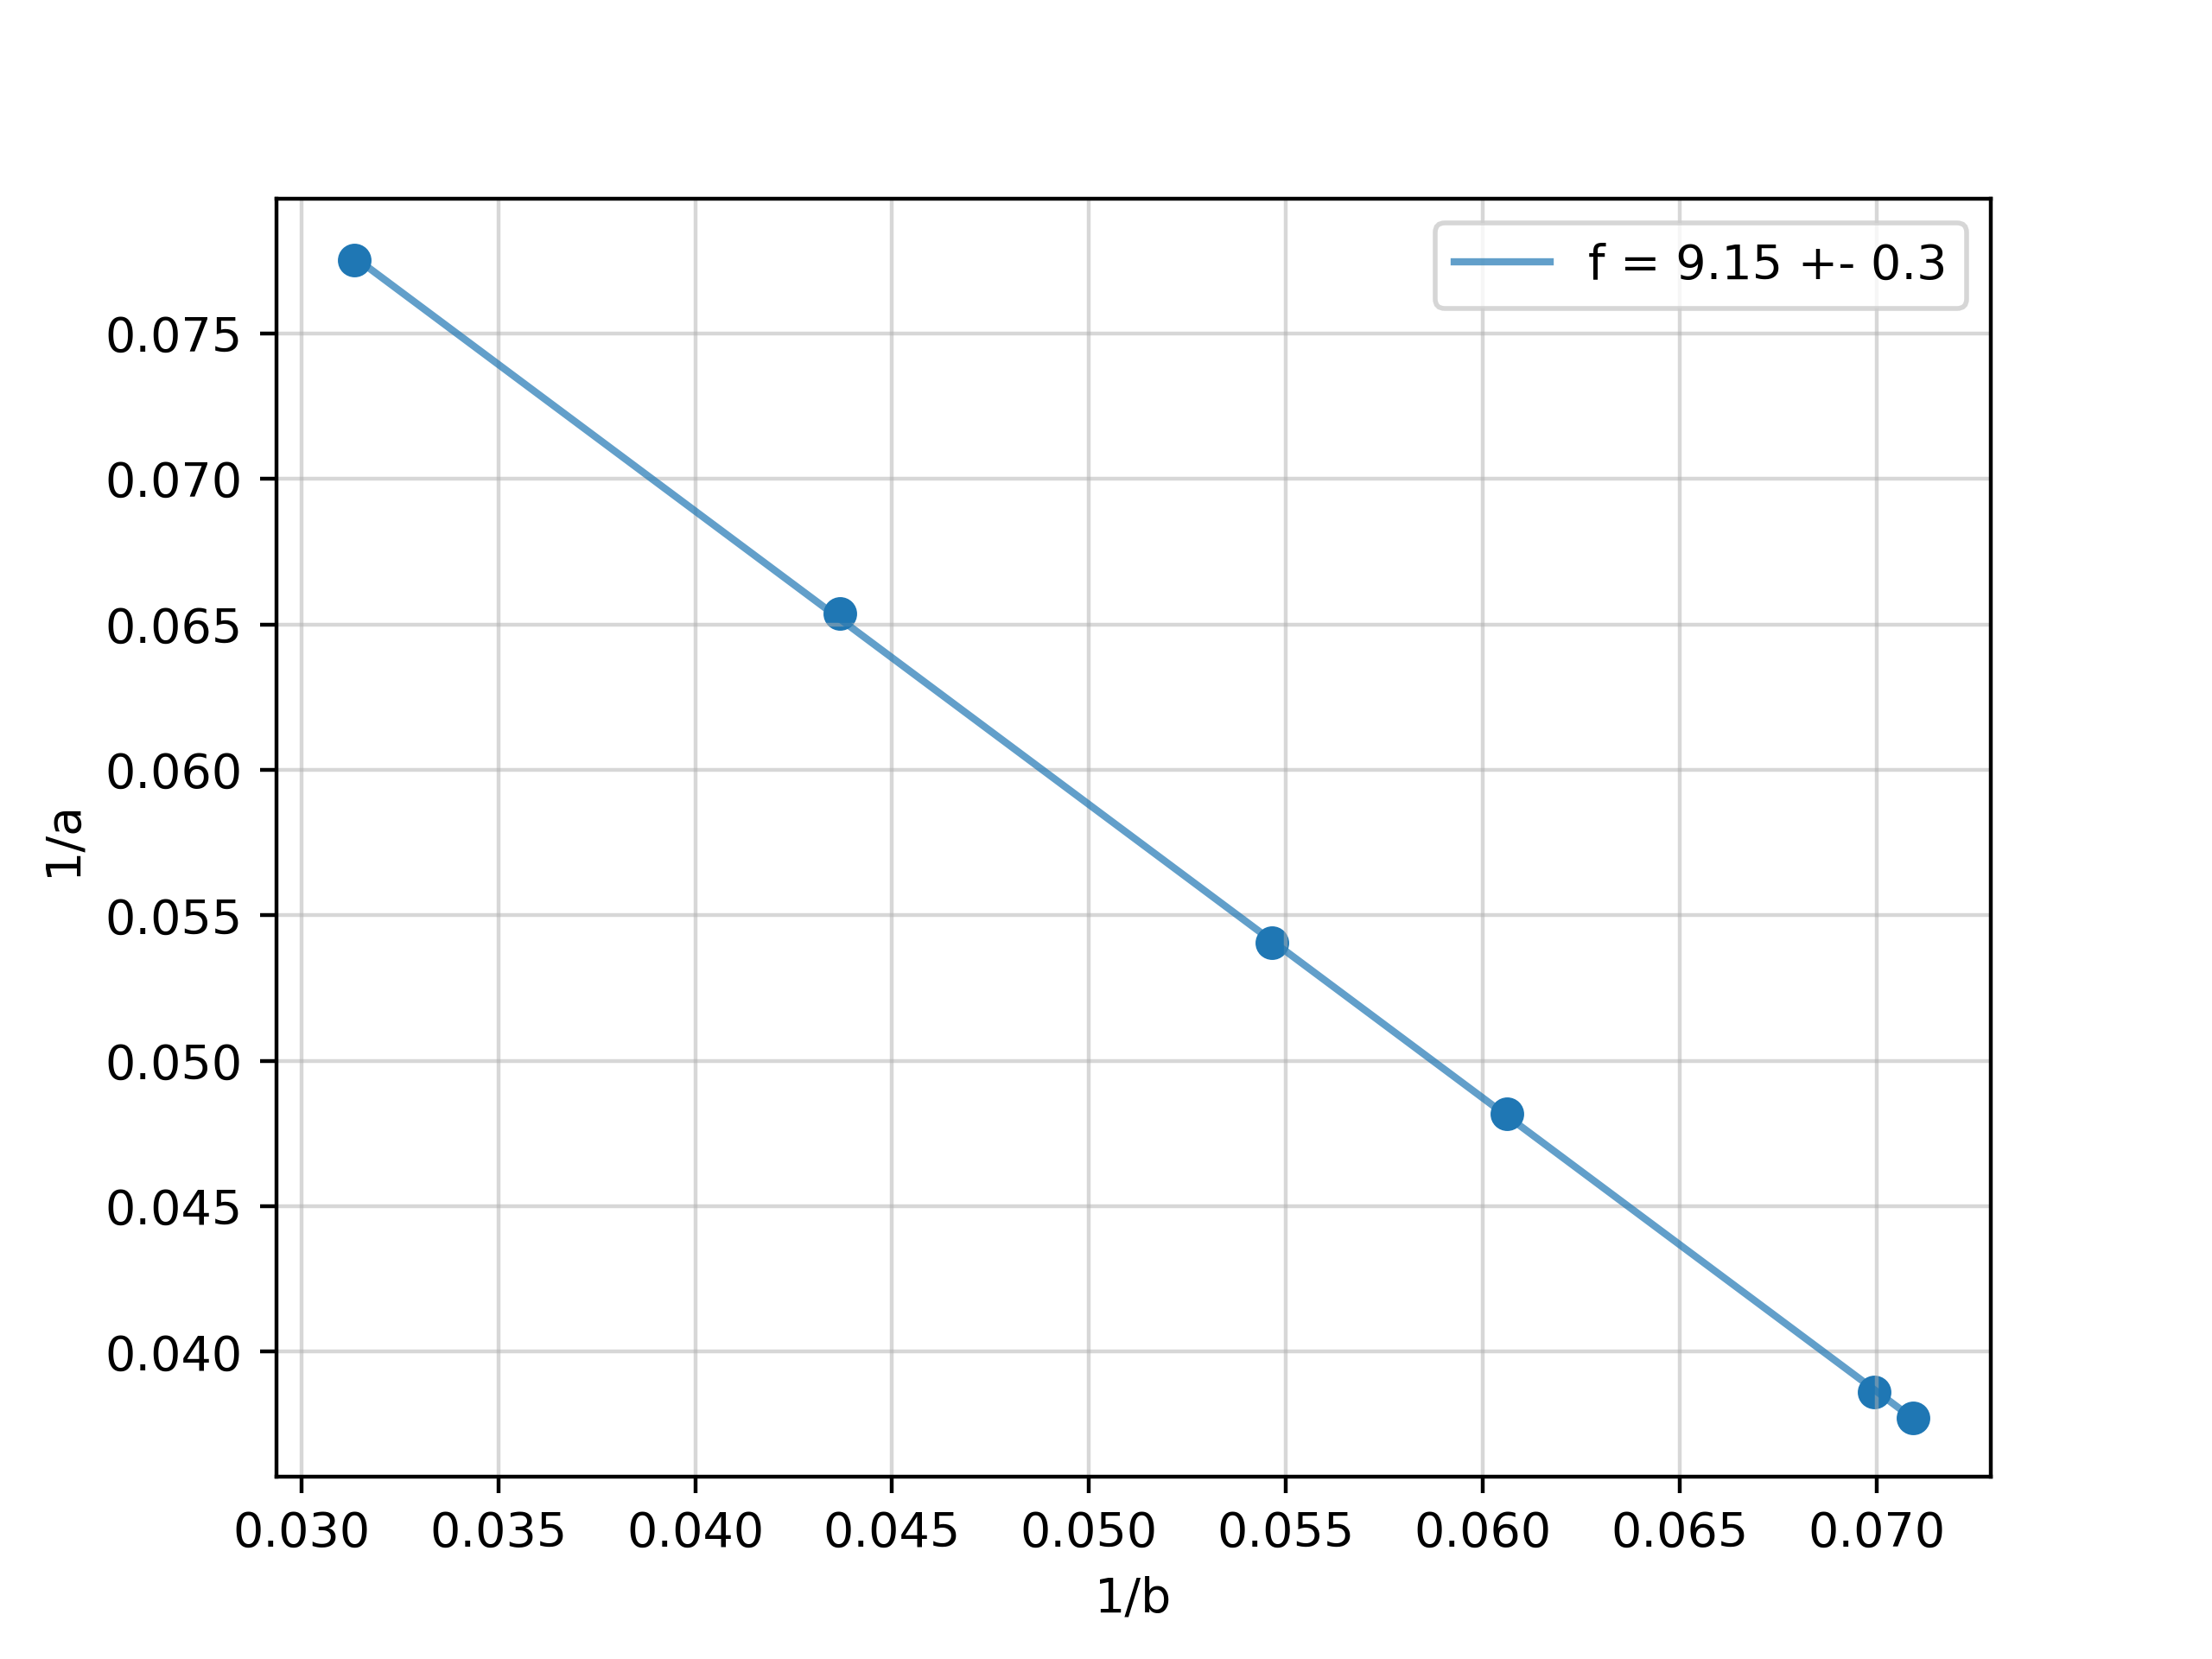
\includegraphics[width=1\textwidth]{plot2.png}
    \caption{$f(1/a)$}
    \label{fig:plo2}
\end{figure}
Имеем:
\begin{equation*}
	\boldmath{f_1 = (7,23 \pm 0,6) \text{ см, }
	f_2 = (9,15 \pm 0,3) \text{ см}}
\end{equation*}

\subsection{Определения фокусных расстояний с помощью зрительной трубы}
В данной части работы получаем следующие результаты:
\begin{equation*}
	\boldmath{f_1 = (7,7 \pm 0,2) \text{ см, }
	f_2 = (9,3 \pm 0,2) \text{ см}}
\end{equation*}
Для отрицательной линзы имеем:
\begin{equation*}
	\boldmath{f_3 = (8,1 \pm 0,3) \text{ см, }}
\end{equation*}

\subsection{Определения фокусных расстояний с помощью метода Бесселя}
Решая систему уравнений на $f$ и $\delta$, получаем:
\begin{equation*}
	\boldmath{f_2 = (8,9 \pm 0,5) \text{ см, }
	\delta = (0,9 \pm 0,07) см}
\end{equation*}

\subsection{Моделирование телескопа}
Получаем:
\begin{equation*}
	\frac{y_2}{y_1} = \frac{17}{5} = 3,4
\end{equation*}
\begin{equation*}
	\frac{f_3}{f_2} = \frac{34,8}{9,2} \approx 3,7
\end{equation*}
Как можно видеть, относительная погрешность составляет около 9\%

\section{Выводы}

Приведем сводную таблицу для всех измерений:
\begin{table}[H]
	\centering
	\begin{tabular}{|c|ccc|}
	\hline
			 & \multicolumn{1}{c|}{Форм. тонк. л.} & \multicolumn{1}{c|}{Зрит. Труба}   & Мет. Бесселя  \\ \hline
	Линза, № & \multicolumn{3}{c|}{f, см}                                                               \\ \hline
	1        & \multicolumn{1}{c|}{$7,23 \pm 0,6$} & \multicolumn{1}{c|}{$7,7 \pm 0,2$} & -             \\ \hline
	2        & \multicolumn{1}{c|}{$9,15 \pm 0,3$} & \multicolumn{1}{c|}{$9,3 \pm 0,2$} & $8,9 \pm 0,5$ \\ \hline
	3        & \multicolumn{1}{c|}{-}              & \multicolumn{1}{c|}{$8,1 \pm 0,2$} & -             \\ \hline
	\end{tabular}
	\caption{Сводная таблица}
	\label{tab:tab1}
\end{table}

Полученные значения совпадают в пределах погрешности. Но стоит сказать, что самым точным методом является метод со зрительной трубой, так как он не дает косвенных погрешностей. 

\end{document}